% !TeX encoding = UTF-8
%
% Grafische Oberflächen:
%


%
% Grafische Oberflächen starten auf eigener Seite.
%
\clearpage


\section{Grafische Oberflächen}
\label{NU:GO}

\paragraph*{\underline{Pflicht:}}

\begin{ids}{\gls{PGO}}

	\id[0010] Ein Hauptmenü mit Auswahl zum "challenge" Modus und zum "creative" Modus.
	
	\id[0020] Ein Menü für der "creativ" Modus um sich zwischen dem erstellen eines neuen Knotens, einer neuen Herausforderung und dem Laden eines Knotens zu entscheiden.
	
	\id[0030] Ein Menü in dem man sich aussuchen kann, welcher Knoten geladen werden soll.
	
	\id[0040] Ein Menü in dem man eine neue Herausforderung zusammenstellt.
	
	\id[0050] Ein Menü in dem man eine Herausforderung zu spielen auswählen kann.
	
	\id[1010] Ein Editor, in dem man den Knoten bearbeitet.
	
	\id[1020] Im Editor /PGO\_1010/ eine Spielfläche in dem man den Knoten sieht und bearbeitet.
	
	\id[1030] Im Editor /PGO\_1010/ ein Pausenmenü, in dem man im "creative" Modus speichern und in jedem Modus das bearbeiten beenden kann.
	
	\id[1040] Im Editor /PGO\_1010/ ein Zugang um ins Pausenmenü /PGO\_1030/ zu gelangen.

\end{ids}




\paragraph*{\underline{Optional:}}

\begin{ids}{\gls{OGO}}

	\id[0010] Im Hauptmenü /PGO\_0010/ eine Auswahl um die Credits anzuzeigen.
	
	\id[0020] Ein Menü für verschiedene Spieleinstellungen.
	
	\id[0030] Im Hauptmenü /PGO\_0010/ eine Auswahl um zum Menü für Spieleinstellungen /OGO\_0020/ zu kommen.
	
	\id[0040] Im Einstellungsmenü /OGO\_0020/ ein Untermenü für die Tastaturbelegung.
	
	\id[0050] Im Einstellungsmenü /OGO\_0020/ ein Untermenü für grafische Einstellungen.
	
	\id[0060] Im Einstellungsmenü /OGO\_0020/ ein Untermenü für audio Einstellungen.
	
	\id[0070] Im Einstellungsmenü /OGO\_0020/ ein Untermenü für eine personaliesierte Farbpalette.
	
	\id[1010] Im Pausenmenü /PGO\_1030/ ein Eintrag um das Einstellungsmenü /OGO\_0020/ anzuzeigen.
	
	\id[1020] Ein Menü für verschiedene Render- und Exportfunktionen.
	
	\id[1030] Im Editor /PGO\_1010/ eine Möglichkeit das Rendermenü /OGO\_1020/ aufzurufen.
	
	\id[1040] /OGO\_1030/ ist nur im "crative" Modus und nach bestandener Herausforderung zugänglich.
	
\end{ids}


% ToDo: An sich wäre noch eine direkte Verlinkung auf die Grafiken an der entsprechenden Stelle gut.

%
%
%
\clearpage



%
%
%



\section*{Visualisierungen}








\section{Interaktionsverlauf}

	\begin{longtable}{|p{0.25\textwidth}|p{0.75\textwidth}|}
    \hline
    main menu & Das ist die erste Ansicht, die der Nutzer bekommt. Von hier aus erreicht er alle Bereiche des Programms.\\
    \hline
    creative & Von hier aus startet der Nutzer ein neues Spiel, mit einem einfachem Standardknoten, lädt einen Speicherstand oder startet das erstellen von neuen Herausforderungen (challenges).\\
    \hline
    challenge & Eine Übersicht, der vorhandenen Herausforderungen. Der Nutzer kann nach verschieden Kriterien suchen und sortieren lassen und in einer Vorschau weitere Informationen betrachten.\\
    \hline
    settings & Einstellungen an Grafik, Ton und Steuerung. Außerdem kann die persönliche Farbpalette angepasst werden.\\
    \hline
    credits & Zeigt Infos über die Mitwirkenden an dem Programm und über das Programm selber.\\
    \hline
    
   \end{longtable}
   
   ~\\
    
	\begin{figure}[h]
		\centering
	 	\includesvg[svgpath=./, width = 0.95\textwidth]{menu}
	 	\caption{Hauptmenüeinträge}
	\end{figure}
	
	\clearpage
	~\\
	
	Im Spiel kann der Nutzer auch die {\color{red} Einstellungen} erreichen. Die Menüeinträge in den unterschiedlichen Spielmodi können variieren.

	\begin{longtable}{|p{0.25\textwidth}|p{0.75\textwidth}|}
	
	\hline
	settings & Genau wie aus dem Hauptmenü.\\
	\hline
	save & Speichert den aktuellen Spielstand.\\
	\hline
	quit & Beendet das laufende Spiel. \\
	\hline
	render options & Bietet dem Nutzer verschiedene Möglichkeiten seinen Knoten zu rendern und zu exportieren.\\
	\hline
	
	\end{longtable}
	
	\begin{figure}[!ht]
		  \centering
		  \includesvg[svgpath=./, width = \textwidth]{ingamemenu}
		  \caption{Menü f. Einstellungen während des Spiels.}
	\end{figure}

	
\clearpage


\section{Benutzerinteraktionsmodelle}
	
\clearpage

\subsection{Spielz{"u}ge}

~\\
...

\subsubsection{Beispiele g{"u}ltiger}


\gls{fa:gueltZug}
~\\
...

\subsubsection{Beispiele ung{"u}ltiger Z{"u}ge}

	\begin{figure}[htb]
	  \centering
	  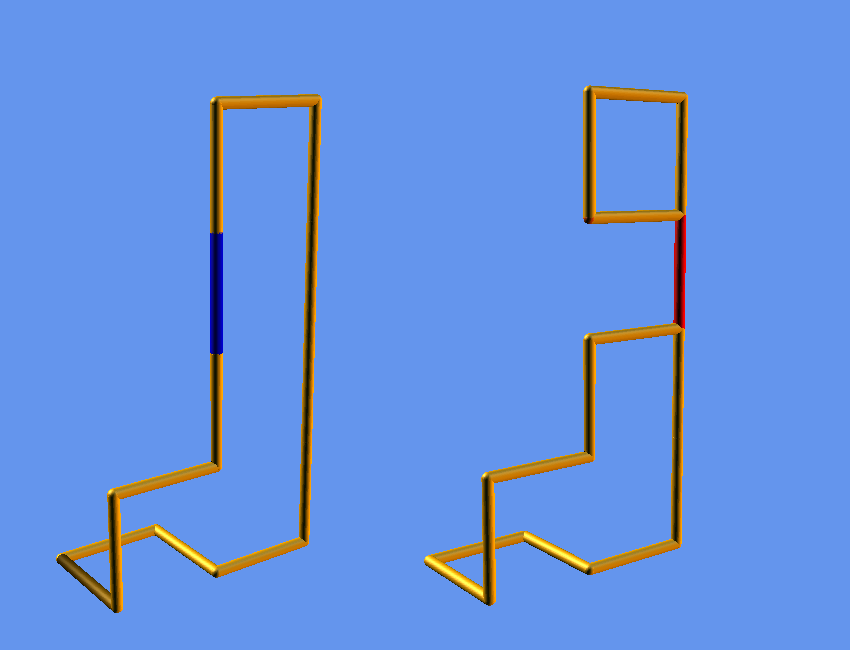
\includegraphics[width = \textwidth]{Inhalt/Nutzung/Grafiken/Grafische_Oberflaechen/Ungueltiger_Zug.png}
	  \caption{Parallele Kantenvereinigung}
	  \label{fig:zug1}
	\end{figure}

Der Knoten auf der linken Seite \ref{fig:zug1} beschreibt eine gültige Spielsituation. Der Spieler wählt eine Kante (blaue Hervorhebung) aus, um einen weiteren Zug vorzunehmen.
Einem Spieler ist es nicht möglich, zwei parallele Kanten (hier: die Blaue und die Rote) zu einer Kante zu vereinen. Das ist ein \gls{fa:ungueltZug}. Der Knoten soll immer aus einem geschlossenen Kreis von Kanten bestehen. Der Knoten auf der rechten Seite \ref{fig:zug1} ist daher eine ungültige Spielsituation.


...

\clearpage



	\begin{figure}[ht]
	% ssetpagelength
	  \centering
	  \includesvg[width = 1.2\textwidth]{inGame}
	  \caption{Interaktionen während eines Spiels (allgemein)}
	\end{figure}



\begin{landscape}

	\begin{figure}[h]
		\centering
	 	\includesvg[width = 1.1\textwidth]{menu}
	 	\caption{Hauptmenüstruktur beginnend mit /PGO\_0010/. Grau hinterlegtes ist Optional.}
	\end{figure}
	
\end{landscape}

\clearpage

\begin{landscape}

	\begin{figure}[h]
		\centering
	 	\includesvg[width = 1.1\textwidth]{ingamemenu}
	 	\caption{Zugriffsmöglichkeiten im Editor /PGO\_1010/. Grau hinterlegtes ist Optional.\\\hspace{\textwidth}
			1: Nur im "creative" Modus\\\hspace{\textwidth}
			2: Nur im "creative" Modus und nach bestandener Herausforderung}
		\label{fig:ingamemenu}
	\end{figure}
	
\end{landscape}
	
\clearpage


%
%
%
\section{Grafische Bedienungs-Oberfl{"a}chen (Mock-Ups)}
	
	\begin{figure}[ht]
	  \centering
	  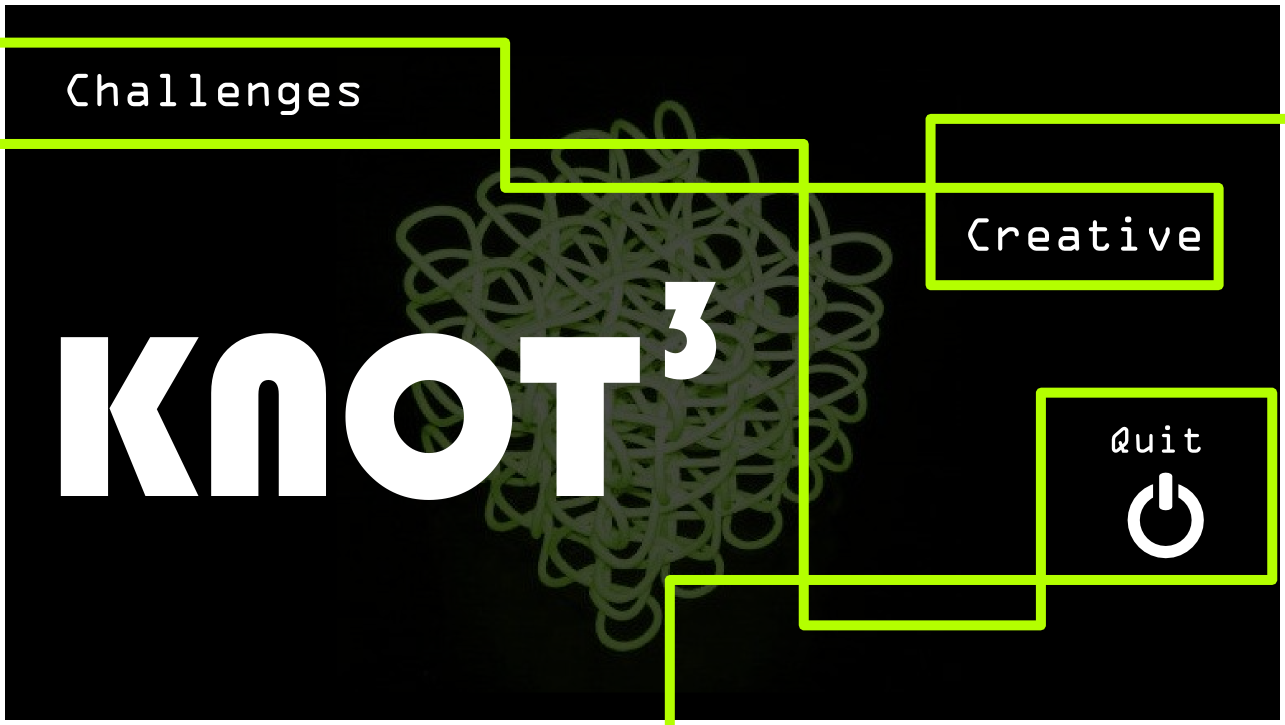
\includegraphics[width = 0.95\textwidth]{Inhalt/Nutzung/Grafiken/Grafische_Oberflaechen/01_Knot3-mainscreen.png}
	  \caption{Mögliches Hauptmenü /PGO\_0010/}
	  \label{fig:mainscreen}
	\end{figure}

	\begin{figure}[!ht]
	  \centering
	  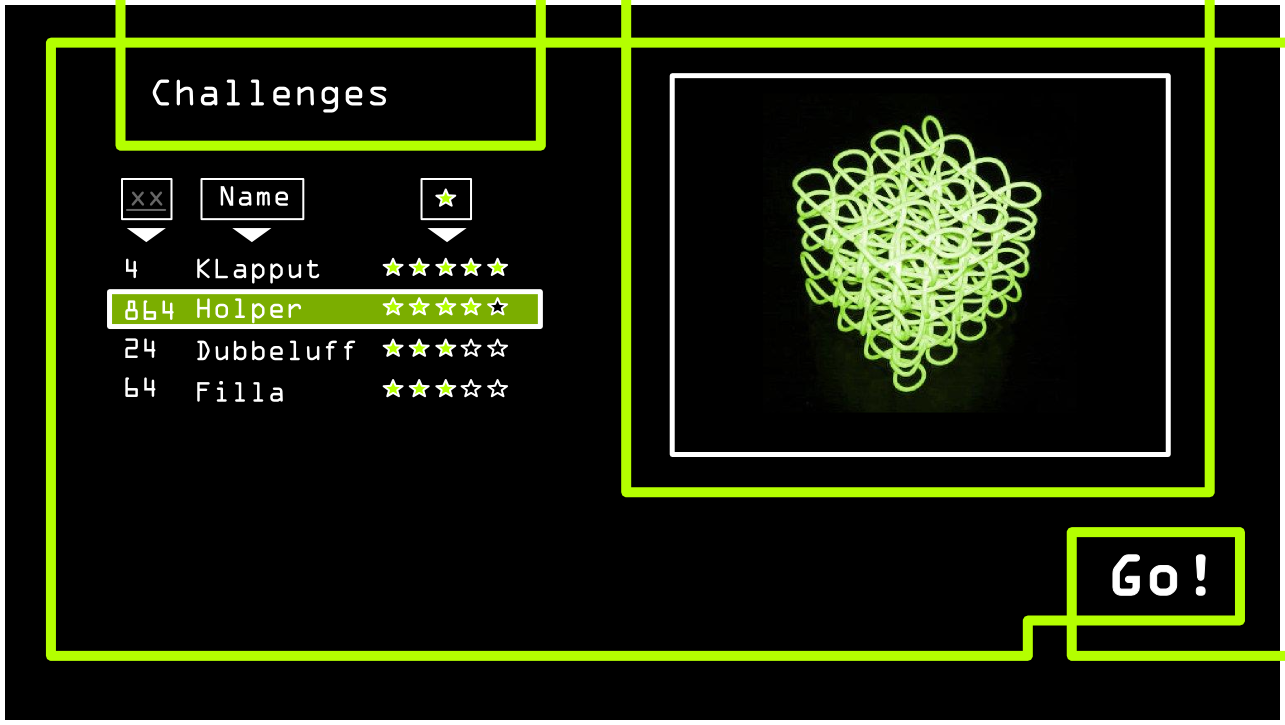
\includegraphics[width = 0.95\textwidth]{Inhalt/Nutzung/Grafiken/Grafische_Oberflaechen/04_Knot3-select-Challenge.png}
	  \caption{Auswahlmenü für die Herausforderungen /PGO\_0050/, mit Ausschnitt der Auswahlliste}
	  \label{fig:selCh}
	\end{figure}
	
	\begin{figure}[ht]
	  \centering
	  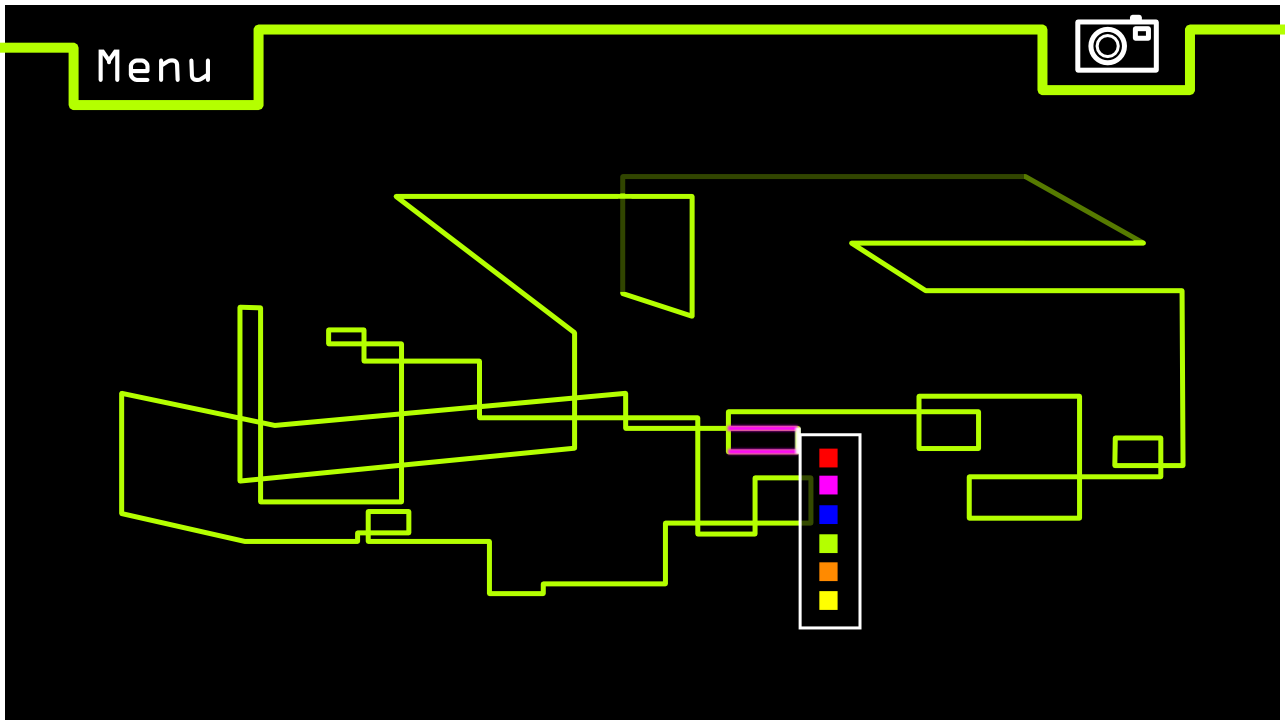
\includegraphics[width = 0.95\textwidth]{Inhalt/Nutzung/Grafiken/Grafische_Oberflaechen/05_Knot3-Colour-select.png}
	  \caption{Editoransicht /PGO\_1010/ mit geöffneter Farbauswahl zum Kanten einfärben /OFA\_200/.}
	  \label{fig:chooseC}
	\end{figure}
	
	\begin{figure}[ht]
	  \centering
	  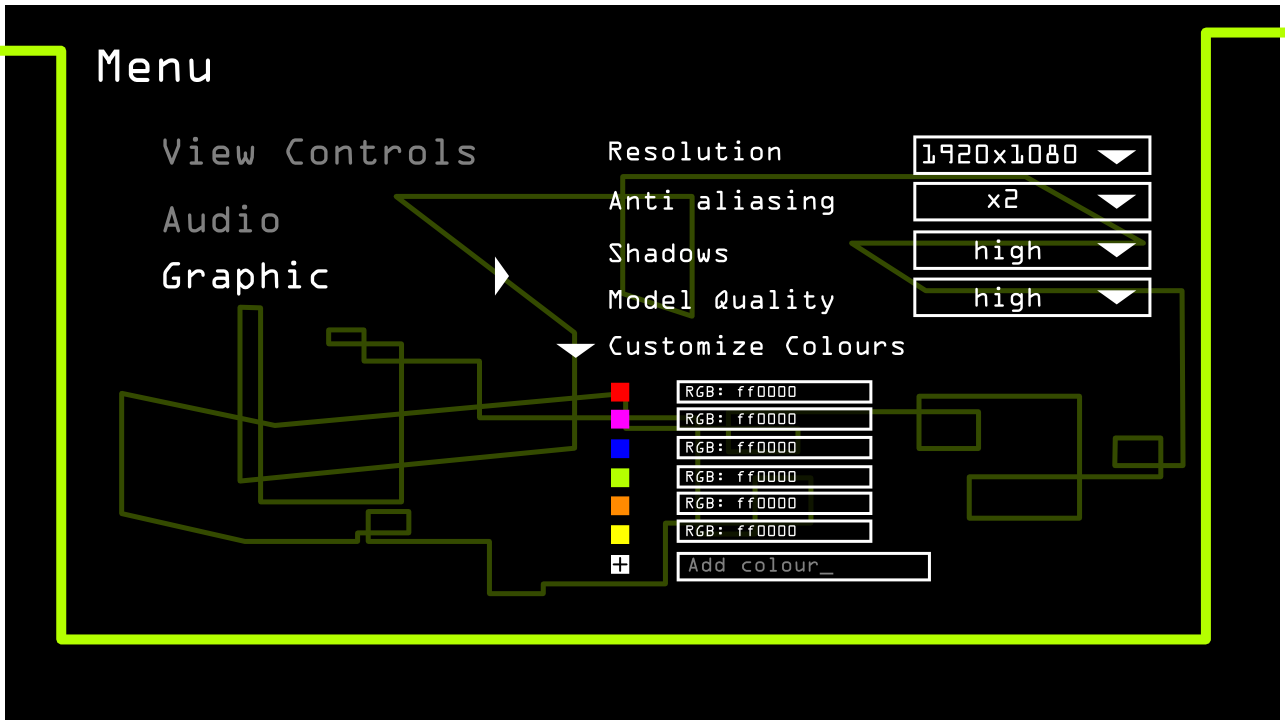
\includegraphics[width = 0.95\textwidth]{Inhalt/Nutzung/Grafiken/Grafische_Oberflaechen/08_Knot3-menu-graphics.png}
	  \caption{Mögliches Einstellungsmenü mit geöffnetem Untermenü für die Grafikeinstellungen. /OGO\_0020/ und /OGO\_0050/}
	  \label{fig:setGFX}
	\end{figure}
	
	\begin{figure}[ht]
	  \centering
	  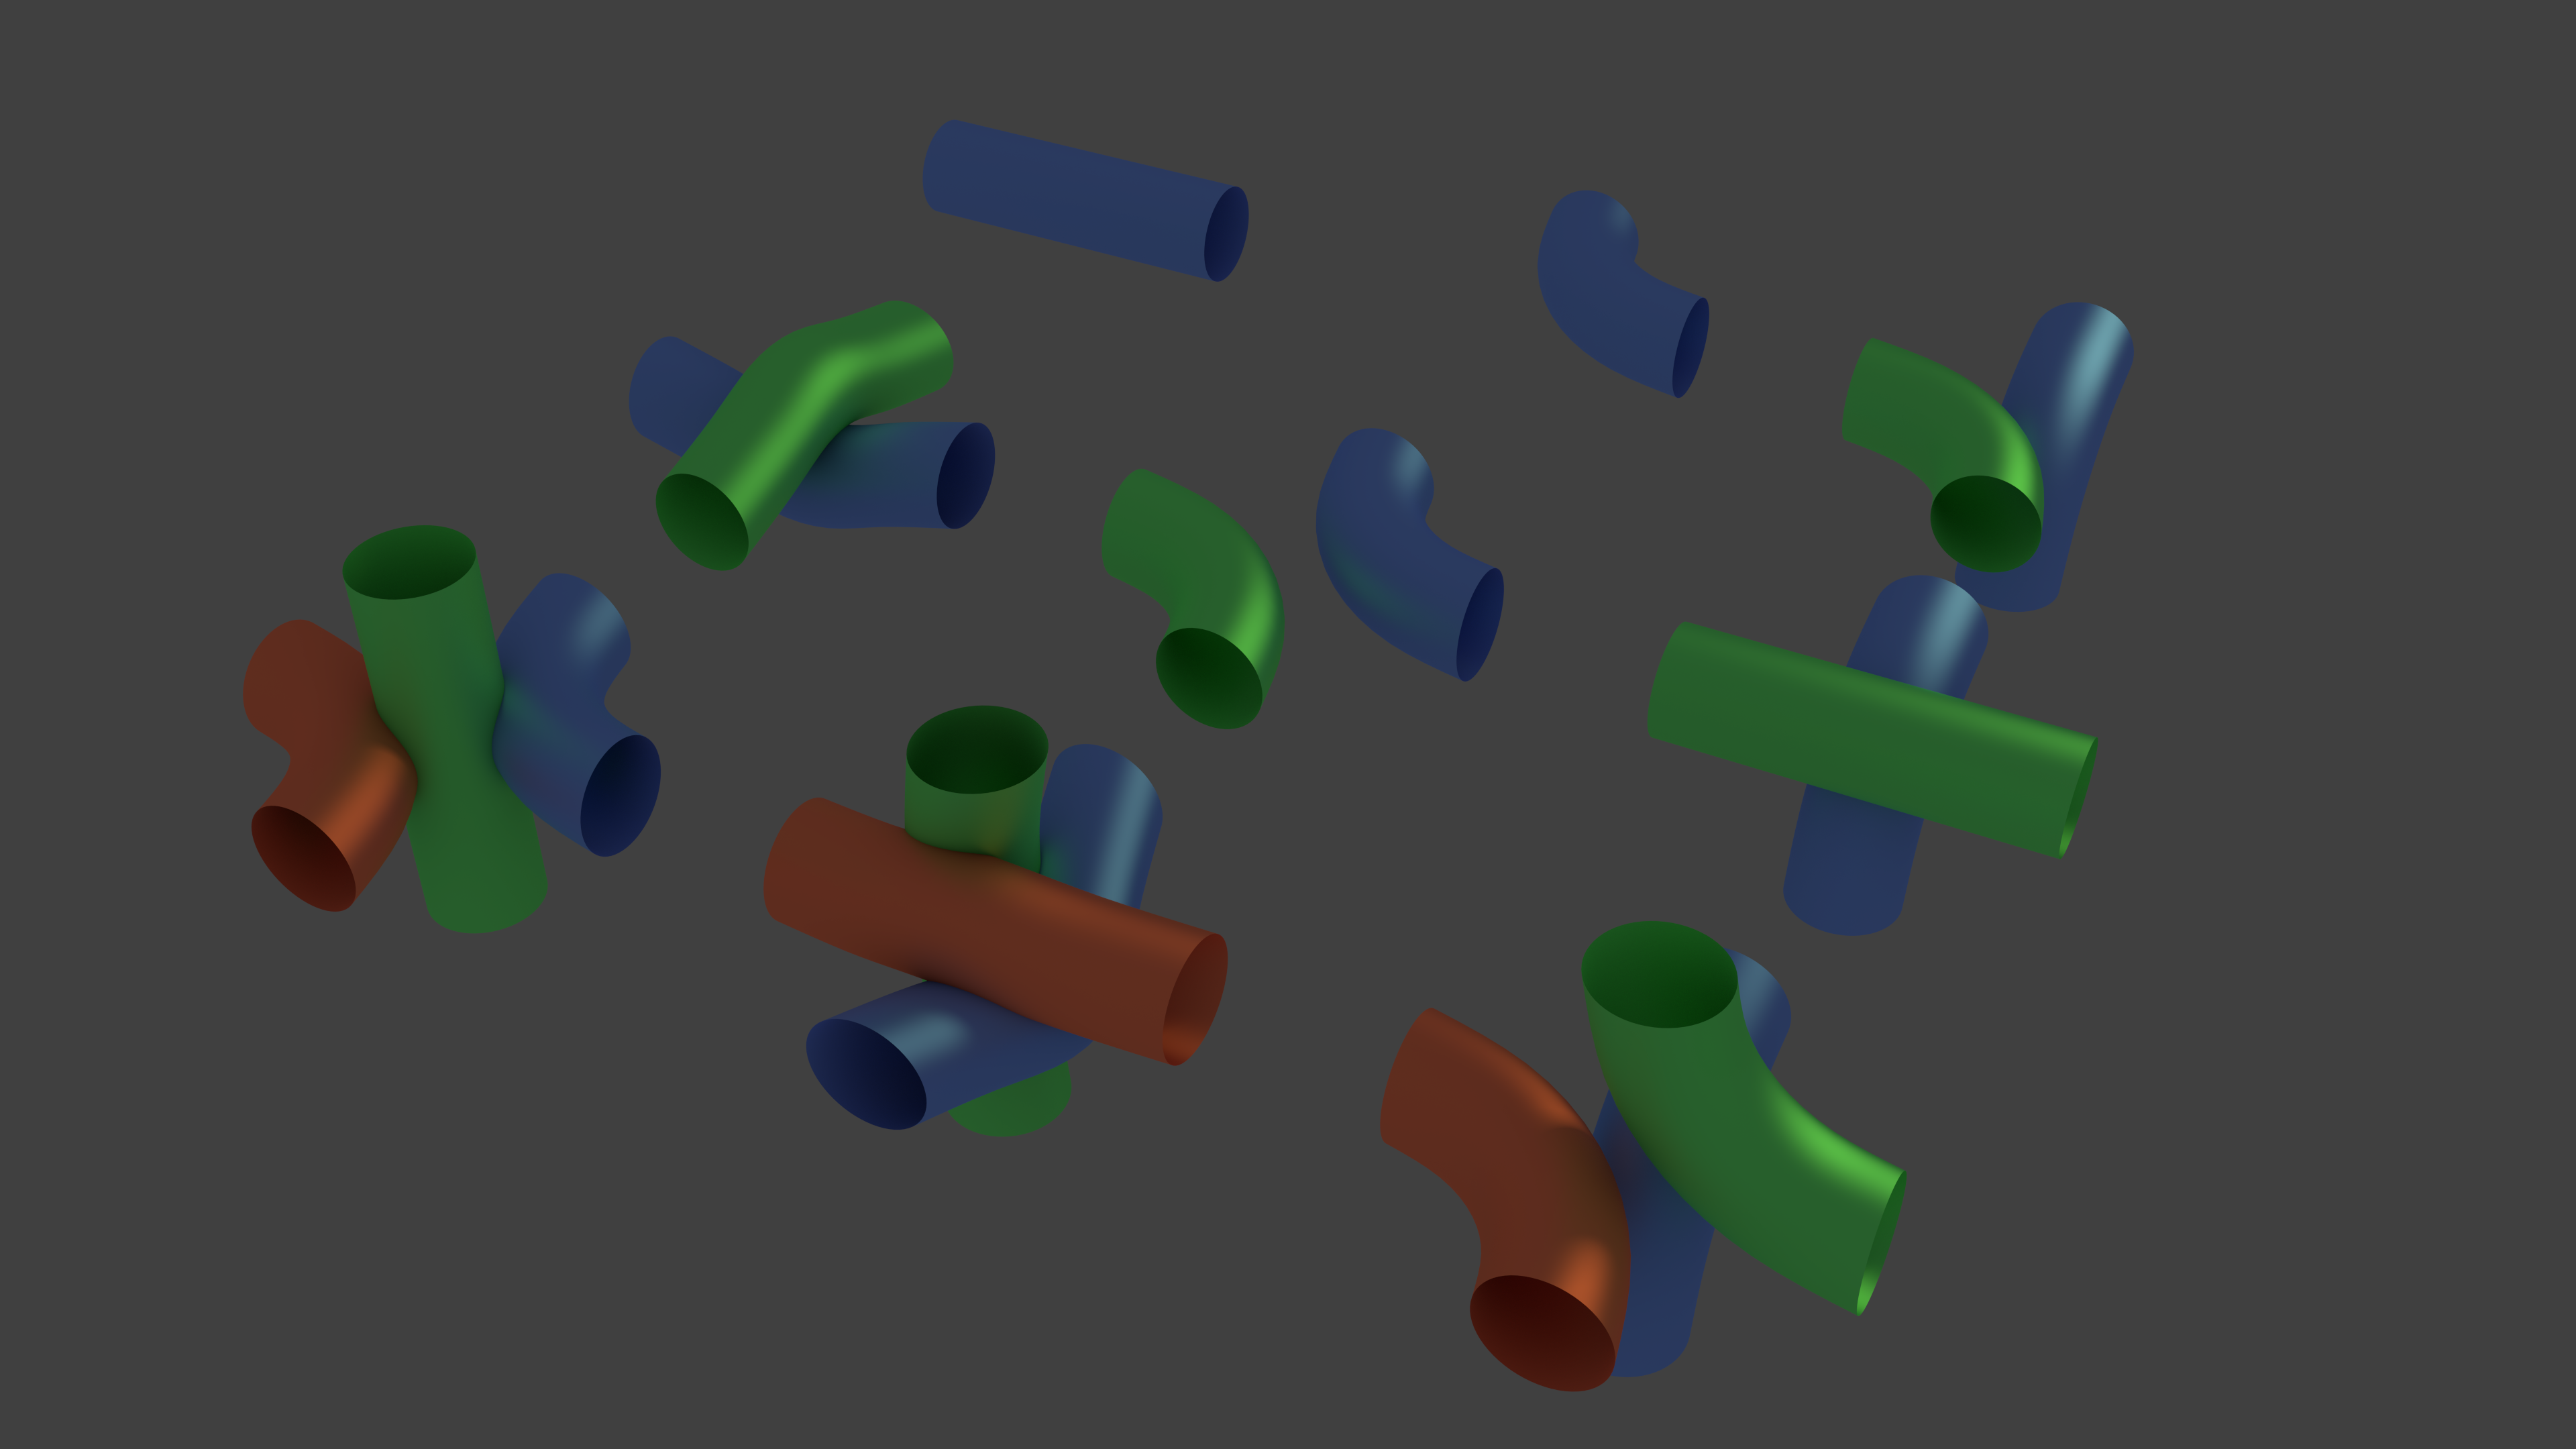
\includegraphics[width = 0.95\textwidth]{Inhalt/Nutzung/Grafiken/Grafische_Oberflaechen/Pipes2.png}
	  \caption{Verschiedene Übergänge für die Kanten}
	  \label{fig:pipes2}
	\end{figure}
	
	

